\section{Szalinski: Decompiling CAD into Structured Programs}
\label{sec:szalinski}

\newcommand{\cadilac}{Caddy\xspace}
\newcommand{\caddy}{Caddy\xspace}
\newcommand{\mtoc}{Mesh-to-CSG\xspace}
\newcommand{\csg}{\ensuremath{\mathit{csg}}\xspace}
\newcommand{\fuel}{\ensuremath{\mathit{fuel}}\xspace}
\newcommand{\affine}{\textsf{Affine}\xspace}
\newcommand{\binop}{\textsf{Binop}\xspace}
\newcommand{\mesh}{\textsf{Mesh}\xspace}
\newcommand{\fold}{\textsf{Fold}\xspace}
\newcommand{\foldu}{\textsf{Foldunion}\xspace}
\newcommand{\foldi}{\textsf{Foldinter}\xspace}
\newcommand{\map}{\textsf{Map2}\xspace}
\newcommand{\maptwo}{\textsf{Map2}\xspace}
\newcommand{\maps}{\textsf{Map2}\textsf{s}\xspace}
\newcommand{\mapi}{\textsf{Tabulate}\xspace}
\newcommand{\mapis}{\textsf{Tabulate}\textsf{s}\xspace}
\newcommand{\rpt}{\textsf{Repeat}\xspace}
\newcommand{\rpts}{\textsf{Repeats}\xspace}
\newcommand{\topk}{top-\textit{k}\xspace}
\newcommand{\emp}{\textsf{Empty}\xspace}
\newcommand{\unit}{\textsf{Cuboid}\xspace}
\newcommand{\sph}{\textsf{Sphere}\xspace}
\newcommand{\cyl}{\textsf{Cylinder}\xspace}
\newcommand{\hx}{\textsf{Hexprism}\xspace}
\newcommand{\scale}{\textsf{Scale}\xspace}
\newcommand{\rotate}{\textsf{Rotate}\xspace}
\newcommand{\trans}{\textsf{Translate}\xspace}
\newcommand{\polar}{\textsf{TranslateSpherical}\xspace}
\newcommand{\union}{\textsf{Union}\xspace}
\newcommand{\unions}{\textsf{Unions}\xspace}
\newcommand{\diff}{\textsf{Difference}\xspace}
\newcommand{\inter}{\textsf{Intersection}\xspace}
\newcommand{\hull}{\textsf{Hull}\xspace}
\newcommand{\slist}{\textsf{List}\xspace}
\newcommand{\slists}{\textsf{Lists}\xspace}
\newcommand{\nil}{\textsf{Nil}\xspace}
\newcommand{\cons}{\textsf{Cons}\xspace}
\newcommand{\concat}{\textsf{Concat}\xspace}
\newcommand{\sdo}{\textsf{Do}\xspace}
\newcommand{\undo}{\textsf{Undo}\xspace}
\newcommand{\unpolar}{\textsf{Unspherical}\xspace}
\newcommand{\unsort}{\textsf{Unsort}\xspace}
\newcommand{\ssort}{\textsf{Sort}\xspace}
\newcommand{\unpart}{\textsf{Unpart}\xspace}
\newcommand{\spart}{\textsf{Part}\xspace}
\newcommand{\Semtag}{Inverse transformations\xspace}
\newcommand{\semtag}{inverse transformations\xspace}
\newcommand{\semt}{inverse transformation\xspace}
\newcommand{\semts}{inverse transformations\xspace}

\lstdefinestyle{caddy}{
  basicstyle=\sffamily,
  columns=flexible,
  showstringspaces=false,
  mathescape,
  escapechar=|,
}

\begin{figure}
  \centering
  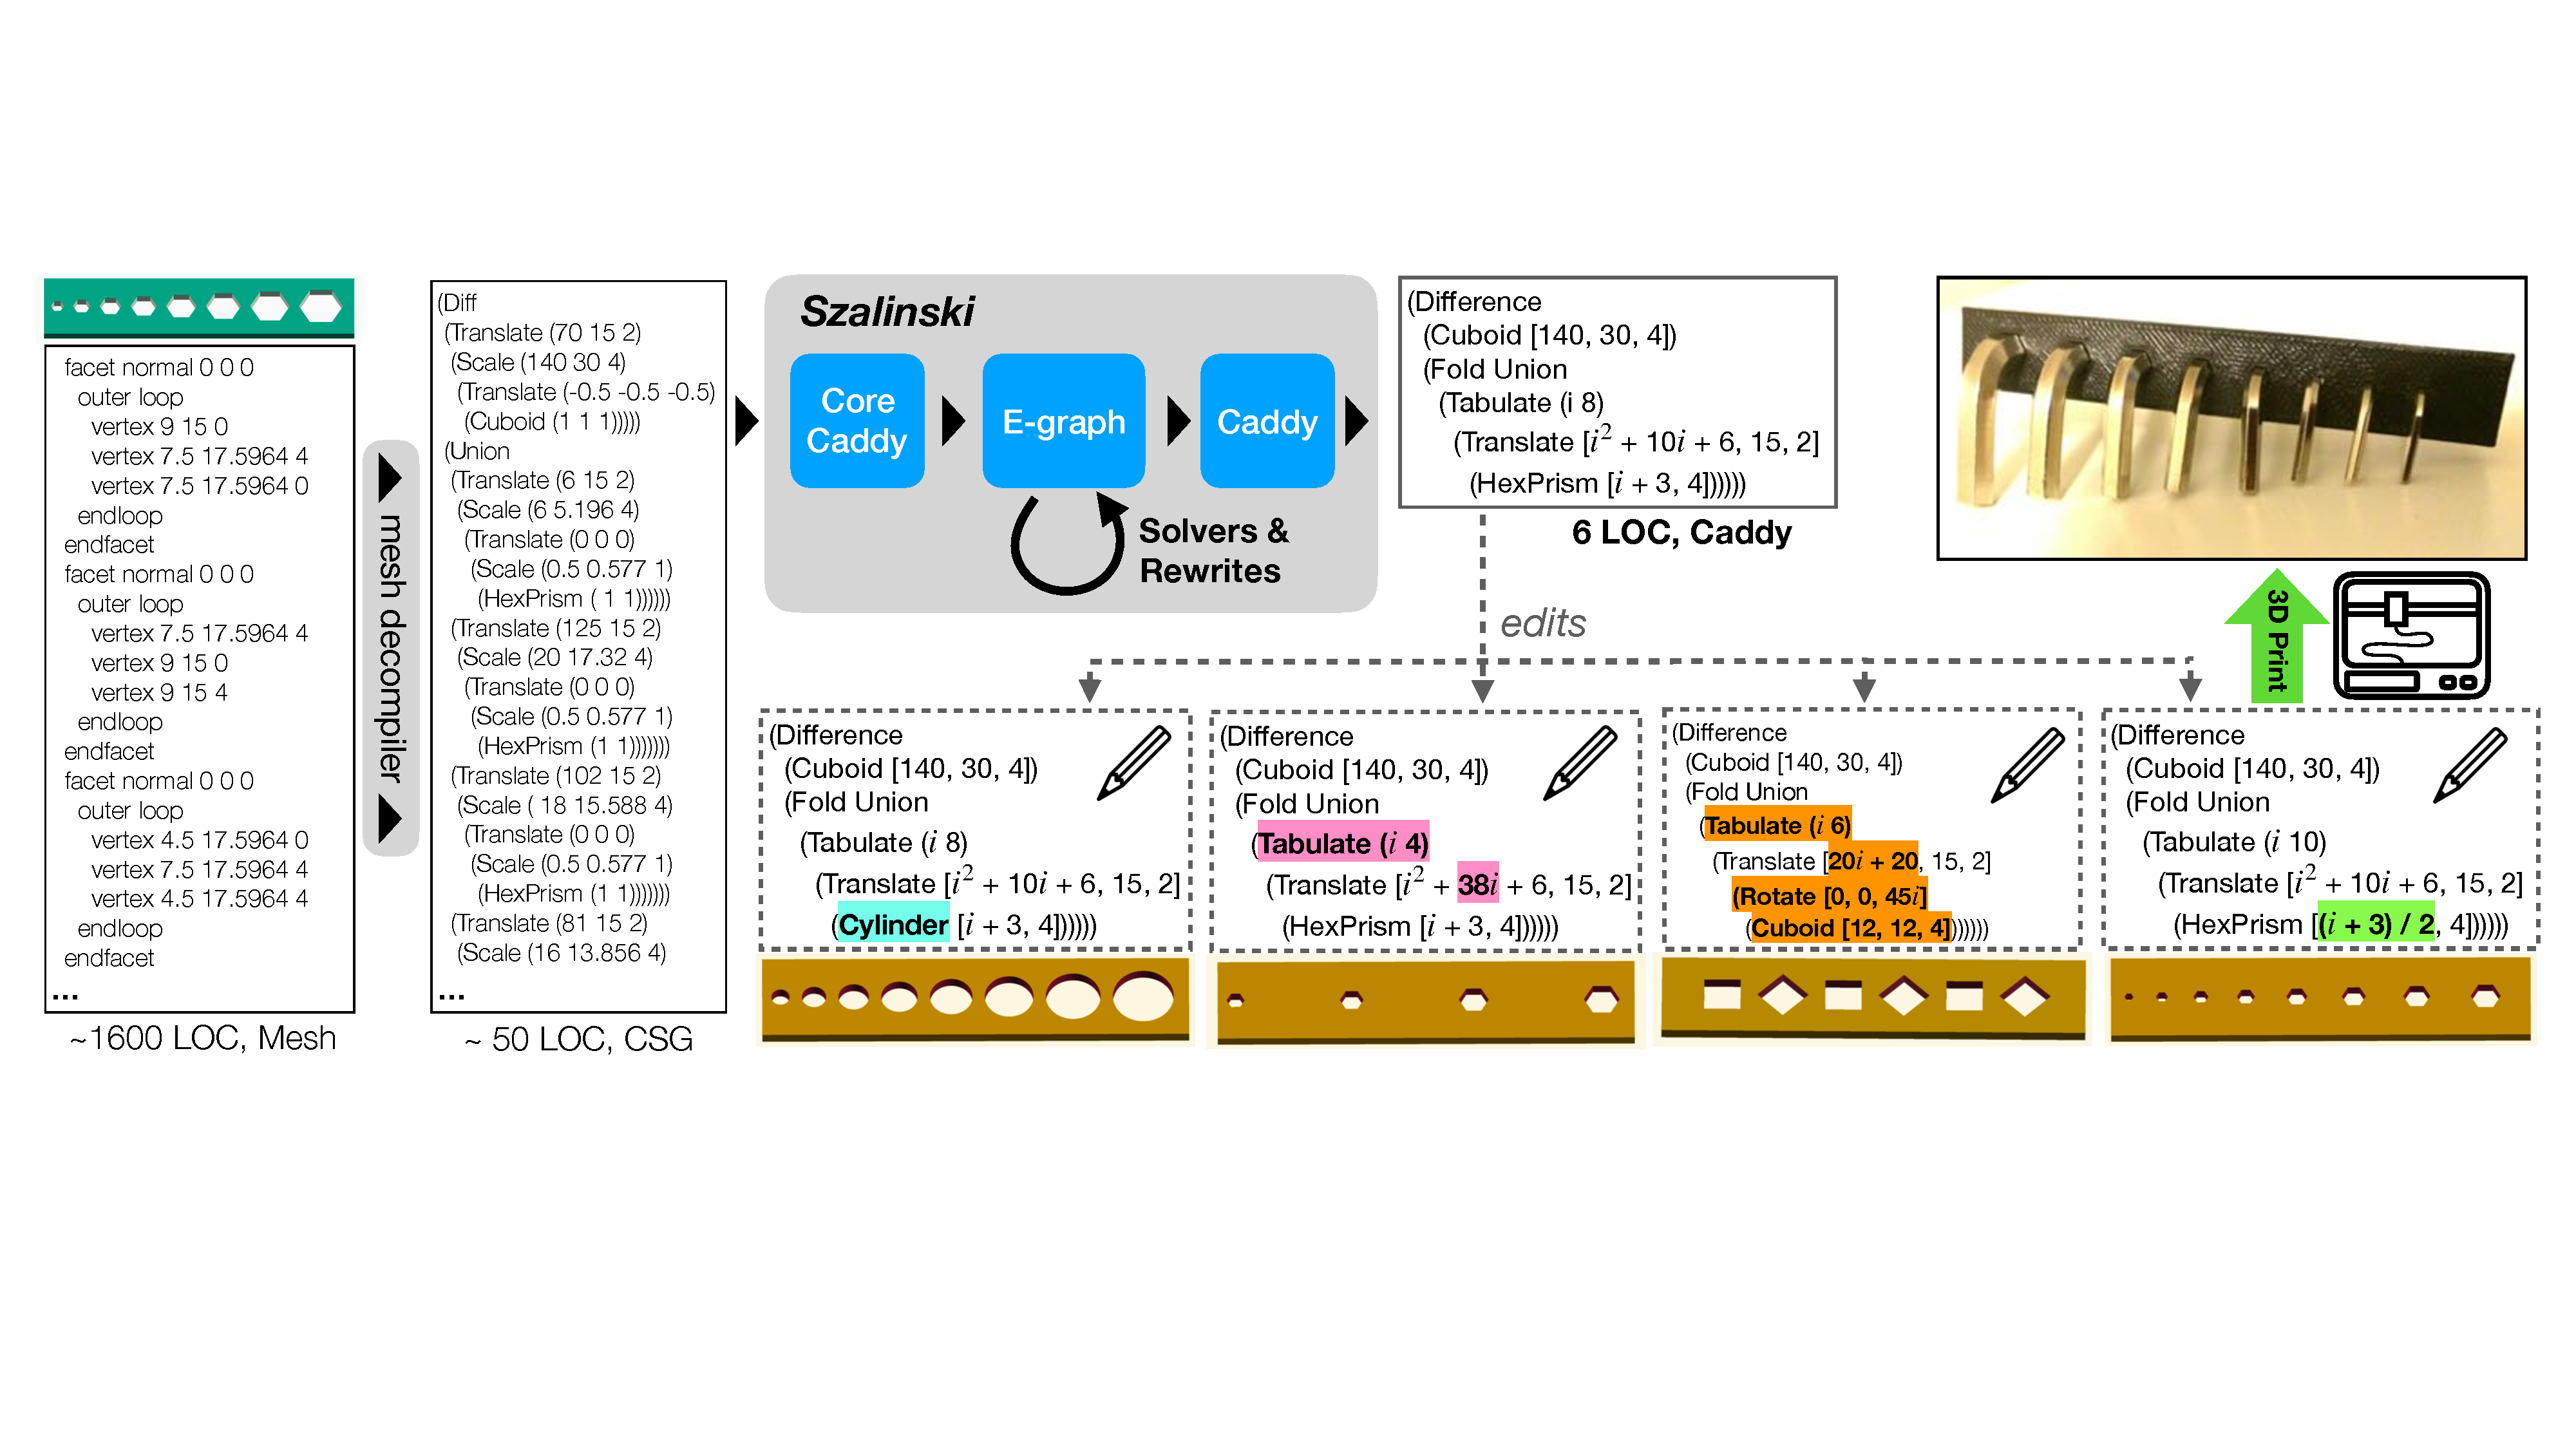
\includegraphics[width=\linewidth]{sz-overview}
  \caption[Szalinski decompiles flat CSG into structured CAD]{
  (Figure from Nandi et.\ al.\ \cite{szalinski})
  Existing mesh decompilers turn
    triangle meshes into flat, computational solid geometry (CSG) expressions.
  %  The size of both mesh and CSG are roughly proportional to
  %    the number of geometric features in the CAD model.
  \sz~\cite{szalinski} takes in these CSG expressions
    in a format called Core Caddy,
    and it synthesizes smaller, structured programs in language called Caddy
    that is enriched with functional-style features.
  This can ease customization by simplifying edits:
    small, mostly local changes
    yield usefully different models.
  The photo shows the 3D printed hex wrench holder after
    customizing hole sizes.
  \sz is powered by \egg's extensible equality saturation, relying on its high
    performance, \eclass analyses, and dynamic rewrites.
  }
  \label{fig:sz-overview}
\end{figure}

Several tools have emerged
  that reverse engineer high level
  Computer Aided Design (CAD) models from polygon
  meshes and voxels~\cite{reincarnate, inverse, shape, csgnet, latex}.
The output of these tools are constructive solid geometry (CSG) programs.
A CSG program is comprised of
  3D solids like cubes, spheres, cylinders,
  affine transformations like scale, translate, rotate
  (which take a 3D vector and a CSG expression as arguments),
  and binary operators like union, intersection, and difference
  that combine CSG expressions.
For repetitive models like a gear, CSG programs can be too long
  and therefore difficult to comprehend.
A recent tool, \sz~\cite{szalinski},
  extracts the inherent structure
  in the CSG outputs of mesh decompilation tools
  by automatically inferring maps and folds (\autoref{fig:sz-overview}).
\sz accomplished this using \egg's extensible equality saturation system,
  allowing it to:

\begin{itemize}

  \item Discover structure using loop rerolling rules.
    This allows \sz to infer functional patterns like
    \texttt{Fold}, \texttt{Map2}, \texttt{Repeat} and
    \texttt{Tabulate} from flat CSG inputs

  \item Identify equivalence among CAD terms that are
    expressed as different expressions by mesh decompilers.
    \sz accomplishes this by using CAD identities.
    An example of one such CAD identity in \sz is
    $e \leftrightarrow \mathit{rotate}~[0 ~ 0 ~ 0] ~ e$.
    This implies that any CAD expression $e$
    is equivalent to a CAD expression that applies
    a rotation by zero degrees about x, y, and z axes
    to $e$

  \item Use external solvers to
    speculatively add potentially profitable
    expressions to the \egraph.
    Mesh decompilers often generate CSG expressions
    that order and/or group list elements in
    non-intuitive ways.
    To recover structure from such expressions,
    a tool like \sz must be able to reorder and regroup
    lists that expose any latent structure

\end{itemize}

\begin{figure}
  \begin{subfigure}[b]{0.48\linewidth}
    \centering
    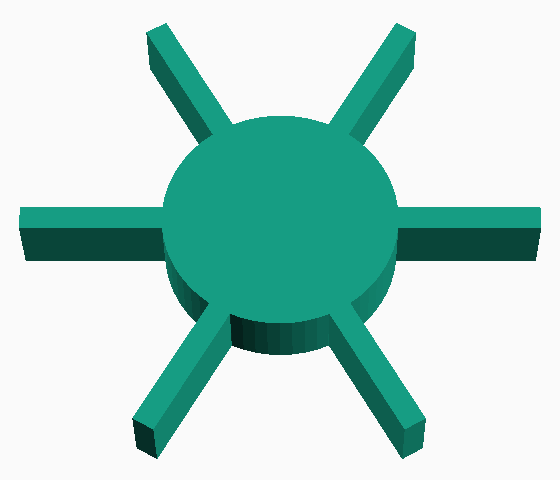
\includegraphics[height=40mm]{sz/shipwheel.png}
    \caption{CAD model of ship's wheel}
    \label{fig:ship-cad}
  \end{subfigure}
  \hfill
  \begin{subfigure}[b]{0.48\linewidth}
    \begin{lstlisting}[style=caddy, xleftmargin=10mm]
(Union
 (Cylinder |[1, 5, 5]|)
 (Fold Union
  (Tabulate (i 6)
   (Rotate |[0, 0, 60 * i]|
    (Translate |[1, -0.5, 0]|
     (Cuboid |[10, 1, 1]|))))))
    \end{lstlisting}
    \caption{\caddy program}
    \label{fig:ship-prog}
  \end{subfigure}
  \vspace{1em}

  \begin{subfigure}{\linewidth}
    \begin{lstlisting}[style=caddy, xleftmargin=25mm]
(Union
 (Cylinder |[1,5]|)
 (Union
  (Rotate |[0,0,0]|   (Translate |[1,-0.5,0]| (Cuboid |[10,1,1]|)))
  (Rotate |[0,0,60]|  (Translate |[1,-0.5,0]| (Cuboid |[10,1,1]|)))
  (Rotate |[0,0,120]| (Translate |[1,-0.5,0]| (Cuboid |[10,1,1]|)))
  (Rotate |[0,0,180]| (Translate |[1,-0.5,0]| (Cuboid |[10,1,1]|)))
  (Rotate |[0,0,240]| (Translate |[1,-0.5,0]| (Cuboid |[10,1,1]|)))
  (Rotate |[0,0,300]| (Translate |[1,-0.5,0]| (Cuboid |[10,1,1]|)))))
    \end{lstlisting}
    \caption{
      Ideal Core \caddy expression that exposes structure
    }\label{fig:ship-csg-good}
  \end{subfigure}
  %%
  \begin{subfigure}{\linewidth}
    \begin{lstlisting}[style=caddy, xleftmargin=20mm]
(Union
  (Rotate    |[0,0,120]|  (Translate |[1,-0.5,0]|   (Cuboid |[10,1,1]|)))
  (Scale     |[10,1,1]|   (Translate |[0.1,-0.5,1]| (Cuboid |[1,1,1]|)))
  (Rotate    |[0,0,300]|  (Translate |[1,-0.5,0]|   (Cuboid |[10,1,1]|)))
  (Scale     |[5,5,1]|    (Cylinder  |[1,1]|))
  (Translate |[-1,0.5,0]|  (Scale     |[-1,-1,1]|    (Cuboid |[10,1,1]|)))
  (Rotate    |[0,0,240]|  (Translate |[1,-0.5,0]|   (Cuboid |[10,1,1]|)))
  (Rotate    |[0,0,60]|   (Translate |[1,-0.5,0]|   (Cuboid |[10,1,1]|))))
    \end{lstlisting}
    \caption{
      Equivalent Core \caddy expression that obfuscates structure
    }\label{fig:ship-csg-bad}
  \end{subfigure}

  \caption{
    \subref{fig:ship-cad} CAD model for a ship's wheel.
    \subref{fig:ship-prog} \caddy features like \mapi express
      repeated design components.
    Such repetition can be obvious in
      Core Caddy \subref{fig:ship-csg-good},
      but existing mesh decompilers
      obfuscate structure \subref{fig:ship-csg-bad}.
  }\label{fig:ship}
\end{figure}

\subsection{Implementation}

Even though CAD is
  different from traditional languages
  targeted by programming language techniques,
  \egg supports \sz's CAD language in a straightforward manner.
\sz uses purely syntactic rewrites to express
  CAD identities and some loop rerolling rules
  (like inferring a \texttt{Fold} from a list of CAD expressions).
Critically, however, \sz relies on \egg's
  dynamic rewrites and \eclass analysis to infer functions
  for lists.

Consider the flat CSG program in \autoref{fig:sz-egg-input}.
A structure finding rewrite first rewrites the flat list of \texttt{Union}s to:
$$\texttt{(Fold Union (Map2 Translate [(0 0 0) (2 0 0) ...] (Repeat Cube 5)))}$$
The list of vectors is stored as \texttt{Cons} elements (sugared above for brevity).
\sz uses an \eclass analysis to track the accumulated lists in a similar style
  to constant folding.
Then, a dynamic rewrite uses an arithmetic solver to rewrite the concrete
  list of 3D vectors in the analysis data
  to \mbox{\texttt{(Tabulate (i 5) (* 2 i))}}.
A final set of syntactic rewrites can hoist the \texttt{Tabulate}, yielding the
  result on the right of \autoref{fig:sz-egg}.
Thanks to the set of syntactic CAD rewrites, this structure finding even works
  in the face of CAD identities.
For example, the original program may omit the no-op
  \texttt{Translate (0 0 0)}, even though it is necessary to see repetitive
  structure.

\begin{figure}
\begin{subfigure}[b]{0.3\linewidth}
  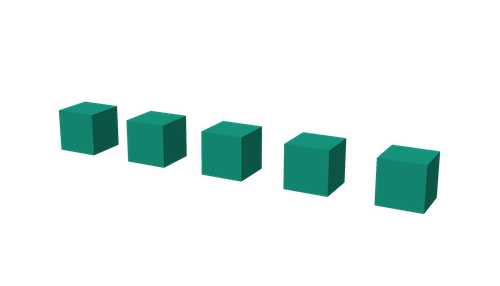
\includegraphics[width=\linewidth]{cubes}
  \caption{Five cubes in a line.}
\end{subfigure}
\hfill
\begin{subfigure}[b]{0.3\linewidth}
  \begin{lstlisting}[language=Rust, gobble=4, basicstyle=\footnotesize\ttfamily]
    (Union
      (Translate (0 0 0) Cube)
      (Translate (2 0 0) Cube)
      (Translate (4 0 0) Cube)
      (Translate (6 0 0) Cube)
      (Translate (8 0 0) Cube))
  \end{lstlisting}
  \caption{Flat CSG input to \sz.}
  \label{fig:sz-egg-input}
\end{subfigure}
\hfill
\begin{subfigure}[b]{0.35\linewidth}
  \begin{lstlisting}[language=Rust, gobble=4, basicstyle=\footnotesize\ttfamily, showlines=true, xleftmargin=5mm]
    (Fold Union
      (Tabulate (i 5)
        (Translate
          ((* 2 i) 0 0)
          Cube)))

  \end{lstlisting}
  \caption{Output captures the repetition.}
  \label{fig:sz-egg-output}
\end{subfigure}
  \caption{
    \sz integrates solvers into \egg's equality saturation as a dynamic rewrite.
    The solver-backed rewrites can transform repetitive lists into
    \texttt{Tabulate} expressions that capture the repetitive structure.
  }
  \label{fig:sz-egg}
\end{figure}

\subsection{Inverse Transformations}

In many cases, the repetitive structure of input CSG expression is further
  obfuscated because subexpressions may appear in arbitrary order.
For these inputs, the arithmetic solvers must first reorder
  the expressions to find a closed form like a \texttt{Tabulate}
  as shown in \autoref{fig:sz-egg}.
However, reordering a list does not preserve equivalence, so adding it to the
  \eclass of the concrete list would be unsound.
\sz therefore introduces \textit{inverse transformations},
  a novel technique that allows solvers to speculatively reorder and regroup list
  elements to find a closed form.
The solvers annotate the potentially profitable expression with the
  permutation or grouping that led to the successful discovery
  of the closed form.
Later in the rewriting process, syntactic rewrites eliminate the inverse
  transformations when possible
  (e.g., reordering lists under a \texttt{Fold Union} can be eliminated).
\egg supported this novel technique without modification.

\subsection{Results}
\sz's initial protoype used a custom \egraph written in OCaml.
Anecdotally, switching to \egg
  removed most of the code,
  eliminated bugs,
  facilitated the key contributions of solver-backed rewrites and inverse transformations,
  and made the tool about $1000 \times$ faster.
\egg's performance allowed a shift from running on small, hand-picked
  examples to a comprehensive evaluation on over 2000 real-world models from
  a 3D model sharing forum~\cite{szalinski}.

%%% Local Variables:
%%% TeX-master: "../thesis"
%%% End: